\chapter{相关技术背景}
本章主要包含三个部分:
1.首先对Top-k算法原理进行了详细的介绍,引出了radix-select算法并阐述了选择它进行实现的理由。
2.介绍了国产AI处理器的编程模型和内存模型。
3.为方便后续验证Top-k算子的可用性,介绍了面向国产AI处理器的pytorch框架。
\section{Top-k算法原理}

如前文所述,在并行Top-k算法领域,已有诸多值得关注的研究成果。在众多成果当中,基于选择的
并行Top-k算法相较于全排序算法具有明显的领先优势。
基于选择的并行Top-K算法包括
QuickSelect [9]、BucketSelect [1]、RadixSelect [1]以及SampleSelect [31]。
其中QuickSelect [9]以快速排序为基础,然而其与传统排序算法的差异在于,
它仅在包含第$K$个元素的子列表上展开迭代操作。此过程通过递归方式持续进行,
直至所选枢轴最终确定为第$K$个元素,并且在前$K$个元素的确定过程中,通过递归收集
逐步达成目标。BucketSelect、SampleSelect和RadixSelect则采用多个枢轴,将候
选元素分配至数十到数百个桶中。BucketSelect的枢轴确定依赖于候选元素的最小值与最
大值;SampleSelect通过对一小部分元素进行采样并排序,以获取更为适宜的枢轴;
RadixSelect与最高有效位基数排序 [14]相似,依据元素的数位特征将元素分配至相应桶中。
而相较于其他三种基于选择的方法,RadixSelect具备若干显著优势:

\begin{enumerate}
\item 在最坏情况下,其时间复杂度为$O(N)$。假设在RadixSelect算法中,一个$r$位数字被分
割为$b$位数字,那么最多仅需$\left\lceil\frac{r}{b}\right\rceil$次迭代。
因此,无论是平均情况还是最坏情况,其时间复杂度均为
$O(\left\lceil\frac{r}{b}\right\rceil N)$。
相比之下,QUICKSELECT在最坏情形下,每次迭代仅能移除一个元素。由此,
处理大约$N$个元素时,$N$次迭代将导致其最坏情况时间复杂度达到$O(N^{2})$。

\item 在GPU上,当采用8位或11位数字(分别对应256个或2048个桶)时,RadixSelect曾展现出高度的
并行性,能够更为有效地削减计算工作量。

\item BucketSelect和SampleSelect在选择枢轴时均需计算输入数据的统计信息,而RadixSelect的枢轴选择与输入数据相互独立。

\end{enumerate}
基于以上原因,本文主要基于RadixSelect算法对Top-k算子进行并行实现。
RadixSelect算法基于基数排序思想,用于在无序数组中找到第k小(或大)的元素,其核心步骤如下:
\begin{enumerate}
    \item {数位分组}:将元素的二进制表示按每连续b位划分为一个数位(digit),从最高有效位开始处理,每次迭代处理一个数位。对于r位元素,共需$\left\lceil\frac{r}{b}\right\rceil$次迭代。
    \item  {计算直方图}:在每次迭代中,提取每个元素当前处理数位的b位并转换为对应的digit值(范围是$[0, 2^{b}-1]$),然后计算直方图以记录每个digit值出现的频率,即直方图的第i个计数器记录digit值等于i的元素数量。
    \item  {计算前缀和}:对直方图计算包含性前缀和(inclusive prefix sum),得到前缀和数组psum。psum[i]表示digit值小于或等于i的元素数量。
    \item  {确定目标数位}:通过前缀和数组找到第k小元素应具有的digit值j,满足psum[j - 1] < K且psum[j] ≥ K。
    \item  {筛选元素}:将digit值小于j的元素确定为当前的Top - k元素,存储其值和索引;digit值大于j的元素可直接丢弃;digit值等于j的元素作为潜在结果存储到候选缓冲区,用于下一次迭代。
    \item  {更新参数}:每次迭代结束后,更新k(减去已确定的Top - k元素数量psum[j - 1])和n(更新为直方图中digit值等于j的元素数量),为下一次迭代做准备。
\end{enumerate}
在算法执行过程中,通过不断迭代上述步骤,逐步缩小候选元素范围,直到找到第k小(或大)的元素。

为了更好的说明上述步骤,下图~\ref{fig:radixselect}介绍了如何从9个元素当中获取Top-4个元素。

\begin{figure}[ht]
    \centering
    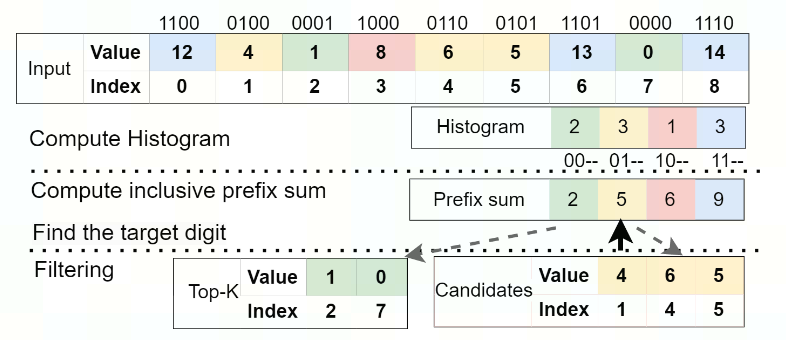
\includegraphics[width=0.8\textwidth]{radixselect.png}
    \caption{RadixSelect流程图}
    \label{fig:radixselect}
    % \note{注:图注的内容不宜放到图题中。}
\end{figure}

对于9个4位元素的列表(以2位为一个数位),第一次迭代计算最高2位的直方图并转换为前缀和,
根据第k小元素(k = 4)的条件确定目标数位为'01',此时digit值为'00'的元素成为部分结果,
digit值为'01'的元素进入候选缓冲区用于下一次迭代,同时更新k和n,继续后续迭代直至找到最终的Top - k元素。





\section{PuDianNao处理器概述}


\section{面向国产AI处理器的pytorch框架}


\section{本章小结}
